\documentclass[11pt,a4paper]{article}
\usepackage[margin=24mm]{geometry}\usepackage{fontspec,unicode-math,booktabs,graphicx,hyperref}
\setmainfont{STIXGeneral}\setmathfont{STIX Two Math}
\title{Complete Mathieu geometry census:\\manuscript and computational costs}
\author{Human Compression project}\date{}
\begin{document}\maketitle
The original is Leemans--Rowley, \emph{Rank three residually connected
geometries for $M_{22}$, revisited}, Electronic Journal of Combinatorics
17 (2010), N4 (register L073). All nine pages are counted. The accepted
replacement gives the corrected complete 81 rank-two and 431 rank-three
classes, with all 431 literal source-row dispositions. It does not recover
the unavailable historical \texttt{geo[]} identities. The 48-page
Kılıç--Rowley predecessor supplies retained notation; it is not a second
newly recovered original.

\paragraph{The complete written comparison.}
For complete raw extraction in NFC, counting characters without whitespace,
\[
 R_{\rm written}=\frac{13736}{5516+(13178+9480+13204)}
 =\frac{13736}{41378}=0.331964.
\]
The replacement is longer in this coordinate. All companion papers are
part of the application: the ten-page class tables and nine-page source-row
tables are not free outputs. The whole common paper is paid once. No earlier
umbrella or another application is used without payment.
\begin{center}\begin{tabular}{lrr}\toprule
Complete document&Pages&Characters\\\midrule
Original L073&9&13736\\
Common theory $U$&2&5516\\
Main application&5&13178\\
All class tables&10&9480\\
All source-row dispositions&9&13204\\
Complete seven-program appendix&11&31244\\\bottomrule
\end{tabular}\end{center}
\paragraph{Required computation and the conditional comparison.}
Both computational routes pay the two complete JSON inputs: 48686
characters, or 83,965 literal file bytes. With the whole printed program
appendix the separate comparison is
$13736/(41378+31244+48686)=0.113232$.
Using the seven whole raw programs instead gives
$13736/(41378+30489+48686)=0.113942$.
The program representations are alternatives; the JSON is required in both.
There is no complete printed-data substitute or pruning of historical rows.

After acquiring \emph{the whole common paper, all seven programs, both
full JSON inputs and all retained premises}, the local application costs
35862 characters across all 24 pages:
\[
 r\mid(U,\mathrm{programs},\mathrm{data})=13736/35862=0.383024.
\]
This conditional comparison also shows an expansion; it is not a standalone
whole-topic saving. The seven programs are required mathematical inputs,
not merely sample diagnostics. The three auxiliary scripts and ten generated
outputs remain inventoried separately, and no Lean formalization is claimed.
\newpage
\begin{center}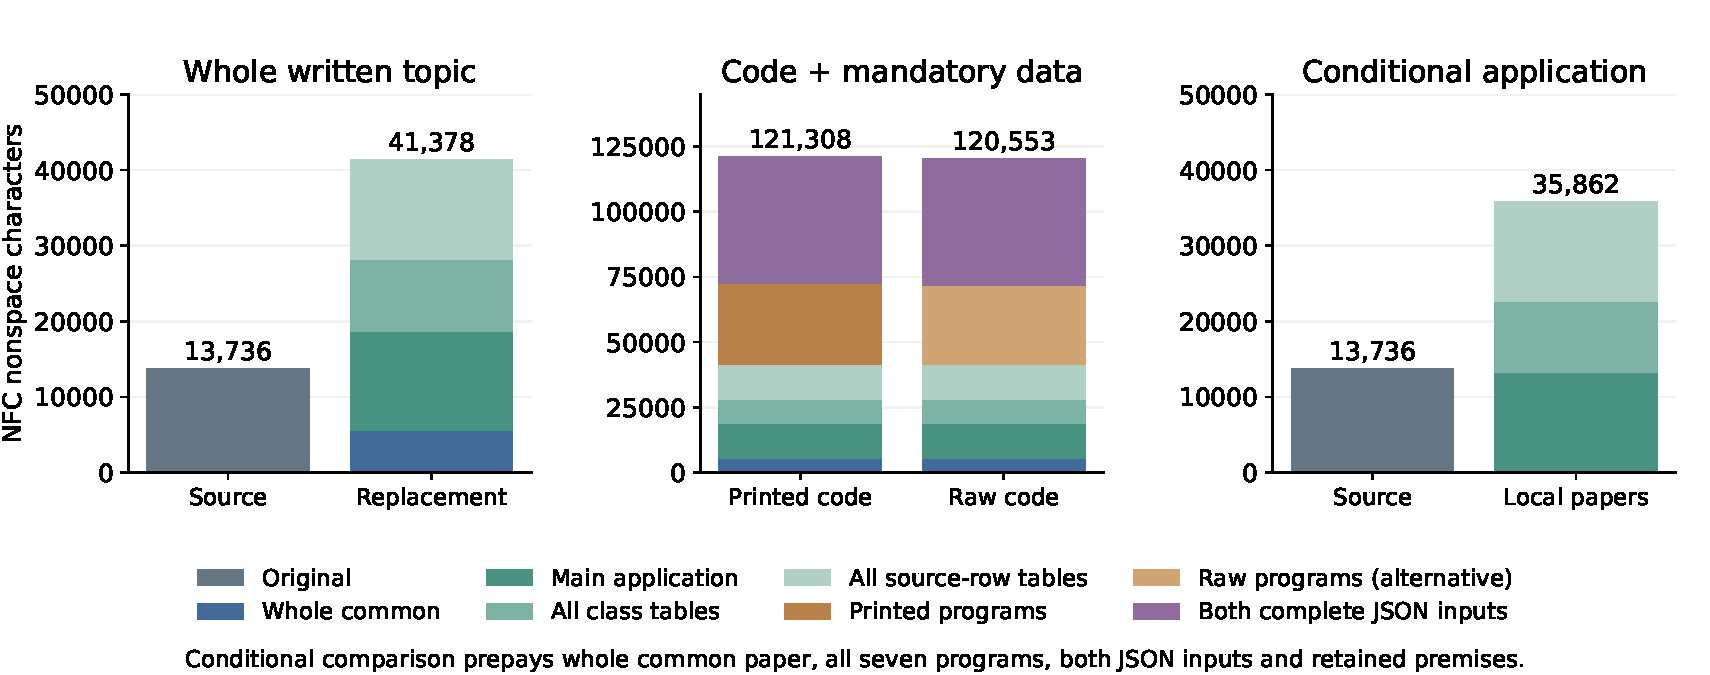
\includegraphics[width=\textwidth]{costs.pdf}\end{center}
\vspace{-4mm}
\begin{center}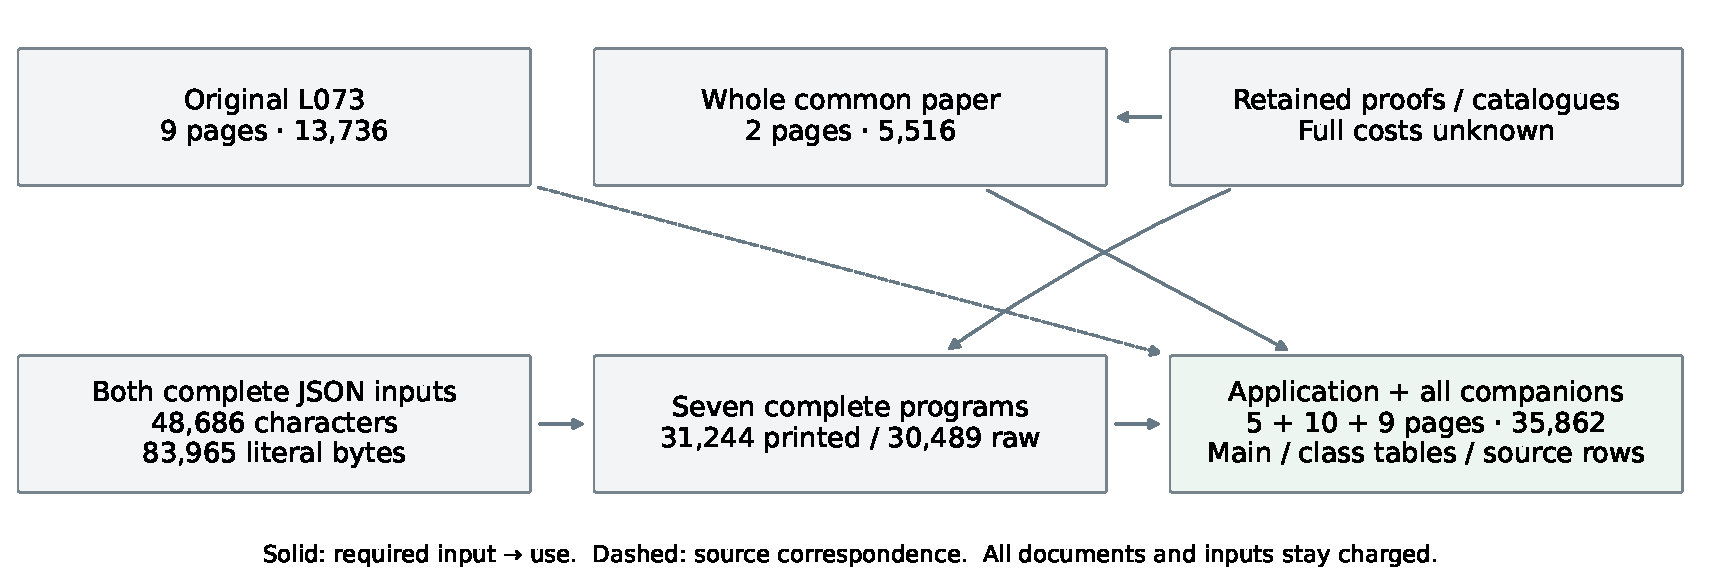
\includegraphics[width=\textwidth]{document_graph.pdf}\end{center}
\vspace{-4mm}
The graph describes complete-document acquisition, not a minimal theorem
DAG. All application companions remain in every written denominator. The
three auxiliary scripts contain 20,542 literal bytes (18689 nonspace
characters); the ten generated outputs contain 1,567,120 bytes (838566
characters). Some outputs feed later pipeline stages; they are not charged
a second time as independent external inputs. Their separate costs remain
available without discount.

\paragraph{Unit and encoding sensitivities.}
Complete raw NFC coordinates are:
\begin{center}\small\begin{tabular}{lrrrr}\toprule
Unit&Written&Printed$+$data&Raw$+$data&Conditional\\\midrule
Whitespace tokens & 0.273 & 0.156 & 0.157 & 0.296 \\
Alphanumeric units & 0.281 & 0.141 & 0.142 & 0.303 \\
Nonspace characters & 0.332 & 0.113 & 0.114 & 0.383 \\
Collapsed-space characters & 0.317 & 0.120 & 0.121 & 0.360 \\
Collapsed-space UTF-8 bytes & 0.305 & 0.120 & 0.120 & 0.347 \\
\bottomrule\end{tabular}\end{center}
All thirty coordinates and 120 exact fractions are retained in JSON/CSV:
five units, NFC and NFKC, for untrimmed, furniture-selected and calibrated
selected text. Selection only removes exact folios and the repeated journal
footer. Six observed script/Fraktur classes account for 472 calibrated
occurrences; raw text is not silently repaired. Normalized text-byte units
are distinct from literal stored-file bytes.

\paragraph{Retained costs and scope.}
Named Mathieu-group identification, complete TomLib catalogue data, exact
GAP/Design/GRAPE algorithms, classical design/Golay facts and predecessor
notation remain explicit premises. Their full proof and catalogue-construction
costs, complete graphic complexity and full formalization cost are unknown,
not zero. The figures are representation lengths, not minimum proof complexity
or research effort. Scientific and input acceptances are reused; this new
arithmetic/reader awaits distinct review and assigns no source, question or
formal credit.
\end{document}
